\documentclass{beamer}
\usepackage[utf8]{inputenc}
\usepackage[english]{babel}
\usepackage[T1]{fontenc}
\usepackage[inline]{asymptote}
\usepackage{pgfplots}
\pgfplotsset{compat=1.5} 
\usepgfplotslibrary{statistics}
\usepackage{slide_helper}

\title[MA205 - Section 3.2]{Measures of Variation}

\newcommand{\textsep}{\vspace{0.5mm}}

\begin{document}
\begin{frame}
\titlepage
\end{frame}

\begin{frame}[fragile]
\begin{example}
Consider the dotplot of waiting times at a bank.
\begin{center}
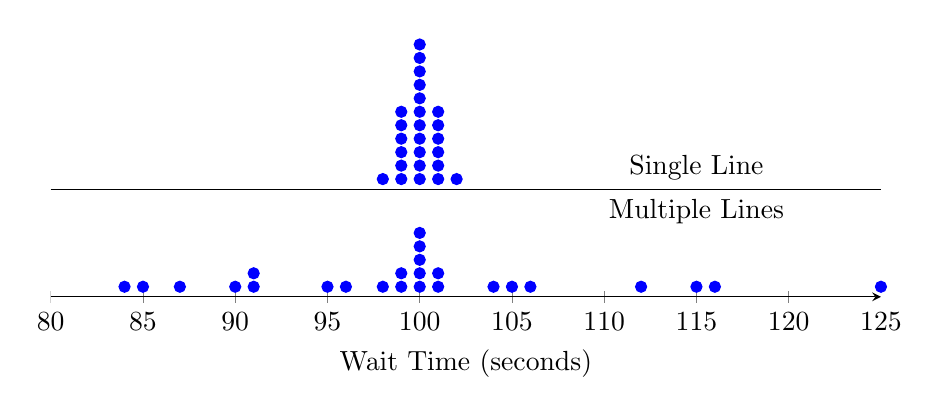
\begin{tikzpicture}
\begin{axis}[
width=\linewidth,
height=5cm,
xlabel={Wait Time (seconds)},
ylabel={},
yticklabels={},
axis y line=none,
axis x line=bottom,
ymin=0,
ymax=20,
xmin=80,
xmax=125,
scatter/use mapped color={
 %draw=mapped color,
 fill=blue,
},
]
\addplot[scatter, only marks, blue, scatter src=y]
coordinates
{
(84, 0.75)
(85, 0.75)
(87, 0.75)
(90, 0.75)
(91, 0.75)
(91, 1.75)
(95, 0.75)
(96, 0.75)
(98, 0.75)
(99, 0.75)
(99, 1.75)
(100, 0.75)
(100, 1.75)
(100, 2.75)
(100, 3.75)
(100, 4.75)
(101, 0.75)
(101, 1.75)
(104, 0.75)
(105, 0.75)
(106, 0.75)
(112, 0.75)
(115, 0.75)
(116, 0.75)
(125, 0.75)
};

\draw (axis cs:80,8) -- (axis cs:125,8);
\draw (axis cs:115,8) node[above]{Single Line};
\draw (axis cs:115,8) node[below]{Multiple Lines};

\addplot[scatter, only marks, blue, scatter src=y]
coordinates
{
(98, 8.75)
(99, 8.75)
(99, 9.75)
(99, 10.75)
(99, 11.75)
(99, 12.75)
(99, 13.75)
(100, 8.75)
(100, 9.75)
(100, 10.75)
(100, 11.75)
(100, 12.75)
(100, 13.75)
(100, 14.75)
(100, 15.75)
(100, 16.75)
(100, 17.75)
(100, 18.75)
(101, 8.75)
(101, 9.75)
(101, 10.75)
(101, 11.75)
(101, 12.75)
(101, 13.75)
(102, 8.75)
};
\end{axis}
\end{tikzpicture}
\end{center}\pause

Both of these data sets have the same mean, but there are clearly different.\pause

\vspace{2mm}
The bank didn't switch to multiple lines because it made them more efficient, nor because customer wait times were reduced, but because customers prefer waiting times with less variation.
\end{example}
\end{frame}

\begin{frame}
\begin{definition}
The \textbf{range} of a set of data values is the difference between the maximum data value and the minimum data value.
\begin{equation*}
\text{Range} = (\text{maximum data value})-(\text{minimum data value})
\end{equation*}
\end{definition}\pause

\begin{block}{Properties}
\begin{itemize}
\item The range is very sensitive to extreme values.\pause
\item Because the range only uses two values it does not reflect the true variation among all of the data values.
\end{itemize}
\end{block}
\end{frame}

\begin{frame}
\begin{example}
Data set 32 \textquote{Airport Data Speeds} in Appendix B includes measures of data speeds of smartphones from four different carriers. The table contains five data speeds, in megabits per second (Mbps), from the data set.

\begin{center}
\begin{tabular}{|l|ccccc|}\hline
\text{Verizon} & 38.5 & \textcolor<3->{blue}{55.6} & 22.4 & \textcolor<3->{red}{14.1} & 23.1\\\hline
\end{tabular}
\end{center}\pause

The range is
\begin{equation*}
\text{Range} = \pause
\textcolor{blue}{55.6}-\textcolor{red}{14.1}\pause
= 41.50~\text{Mbps}
\end{equation*}
\end{example}\pause

\begin{block}{Note}
Just like measures of center, we want to round to one more decimal place that our data contains.
\end{block}
\end{frame}

\begin{frame}
\begin{definition}
The \textbf{standard deviation} of a set of sample values is a measure of how much data values deviate away from the mean.
\end{definition}\pause

\begin{block}{Notation}
\begin{itemize}
\item $s$ is the sample standard deviation.
\item $\sigma$ is the population standard deviation.
\end{itemize}
\end{block}\pause

\begin{block}{Formula}
\begin{equation*}
s = \sqrt{\dfrac{\sum {(x-\bar{x})}^2}{n-1}}
\end{equation*}\pause

A shortcut version that tends to be used by software is
\begin{equation*}
s = \sqrt{\dfrac{n(\sum x^2)-{(\sum x)}^2}{n(n-1)}}
\end{equation*}
\end{block}
\end{frame}

\begin{frame}
\begin{block}{Properties}
\begin{itemize}[<+- | alert@+>]
\item The standard deviation is a measure of how much data values deviate from the mean.
\item The value of the standard deviation is never negative.
\item The value of the standard deviation is only zero when all of the data values are exactly the same.
\item Larger values of s indicate greater amounts of variation.
\item The standard deviation can increase dramatically with one or more outliers.
\item The units of the standard deviation are the same units as the original data values.
\item The sample standard deviation is a \textbf{biased estimator} of the population standard deviation. This means that the values of $s$ for not center around the value of $\sigma$.
\end{itemize}
\end{block}
\end{frame}

\begin{frame}
\begin{block}{Procedure}
For the equation
\begin{equation*}
s = \sqrt{\dfrac{\sum {(x-\bar{x})}^2}{n-1}}
\end{equation*}
use the following general procedure.
\onslide<+->
\begin{description}[<+->]
\item[\textbf{Step 1:}] Compute the mean $\bar{x}$.
\item[\textbf{Step 2:}] Subtract the mean from each data value. (These are called deviations.)
\item[\textbf{Step 3:}] Square each deviations from \textbf{Step 2}.
\item[\textbf{Step 4:}] Add all the squares obtained from \textbf{Step 3}.
\item[\textbf{Step 5:}] Divide the total from \textbf{Step 4} by $n-1$.
\item[\textbf{Step 6:}] Find the square root of the result of \textbf{Step 5}.
\end{description}
\onslide<+->
The result of \textbf{Step 6} is $s$, the standard deviation.
\end{block}
\end{frame}

\begin{frame}
\begin{example}\label{stddevex1}
Data set 32 \textquote{Airport Data Speeds} in Appendix B includes measures of data speeds of smartphones from four different carriers. The table contains five data speeds, in megabits per second (Mbps), from the data set.

\begin{center}
\begin{tabular}{|l|ccccc|}\hline
\text{Verizon} & 38.5 & 55.6 & 22.4 & 14.1 & 23.1\\\hline
\end{tabular}
\end{center}

\onslide<+->
\begin{description}[<+->]
\item[\textbf{Step 1:}] $\bar{x} = \dfrac{38.5 + 55.6 + 22.4 + 14.1 + 23.1}{5} = 30.74~\text{Mbps}$
\item[\textbf{Step 2:}] Deviations:\\
\begin{tabular}{|ccccc|}\hline
7.76 & 24.86 & -8.34 & -16.64 & -7.64\\\hline
\end{tabular}

\item[\textbf{Step 3:}] Squares:
\begin{tabular}{|ccccc|}\hline
60.2176 & 618.0196 & 69.5556 & 276.8896 & 58.3696\\\hline
\end{tabular}
\item[\textbf{Step 4:}] $\text{Sum} = 1083.0520$
\item[\textbf{Step 5:}] $\dfrac{1083.0520}{4}=270.7630$
\item[\textbf{Step 6:}] $s=\sqrt{270.7630}=16.45~\text{Mbps}$
\end{description}
\end{example}
\end{frame}

\begin{frame}
\begin{example}
Data set 32 \textquote{Airport Data Speeds} in Appendix B includes measures of data speeds of smartphones from four different carriers. The table contains five data speeds, in megabits per second (Mbps), from the data set.

\begin{center}
\begin{tabular}{|l|ccccc|}\hline
\text{Verizon} & 38.5 & 55.6 & 22.4 & 14.1 & 23.1\\\hline
\end{tabular}
\end{center}\pause

To use second version of the formula we need to know:
\begin{equation*}
\begin{aligned}
\sum x &= 153.7 \\
\sum x^2 &= 5807.79
\end{aligned}
\end{equation*}\pause

Then,
\begin{equation*}
s = \sqrt{\dfrac{n(\sum x^2)-{(\sum x)}^2}{n(n-1)}} \pause
= \sqrt{\dfrac{5(5807.79)-{(153.7)}^2}{5(5-1)}} \pause
= 16.45~\text{Mbps}
\end{equation*}\pause
This is the same result we found in Example~\ref{stddevex1}.
\end{example}
\end{frame}

\begin{frame}
\begin{block}{Range Rule of Thumb for Identifying Significant Values}
A crude, but simple tool for interpreting the standard deviation.
\begin{description}
\item[\textbf{Significantly low}] values are $\mu-2\sigma$ or lower.
\item[\textbf{Significantly high}] values are $\mu+2\sigma$ or higher.
\item[\textbf{Values not significant}] when between $\mu-2\sigma$ and $\mu+2\sigma$.
\end{description}\pause
This works because for most data sets the vast majority of values fall within two standard deviations of the mean.
\end{block}\pause

\begin{block}{Range Estimate of the Standard Deviation}
A rough estimate of the standard deviation is
\begin{equation*}
s\approx\dfrac{\text{range}}{4}
\end{equation*}
\end{block}
\end{frame}

\begin{frame}
\begin{example}
Using the full data set of Verizon data speeds (Data Set 32 Appendix B)
\begin{equation*}
\begin{aligned}
\bar{x} &= 17.60~\text{Mbps}\\
s &= 16.02~\text{Mbps} 
\end{aligned}
\end{equation*}\pause

Significantly low values are $(17.60-2\cdot 16.02)=-14.44$ Mbps or lower.\pause

\vspace{2mm}
Significantly high values are $(17.60+2\cdot 16.02)=49.64$ Mbps or higher.\pause

\vspace{2mm}
Values that are between $-14.44$ Mbps and $49.64$ Mbps are not significant.
\end{example}\pause

\begin{block}{Note}
Based on this these results, we expect that typical airport Verizon data speeds are between $-14.44$ Mbps and $49.64$ Mbps.
\end{block}
\end{frame}

\begin{frame}
\begin{block}{Standard Deviation of a Population}
A population of size $N$ has standard deviation
\begin{equation*}
\sigma = \sqrt{\dfrac{\sum{(x-\mu)}^2}{N}}
\end{equation*}
\end{block}\pause

\begin{block}{Note}
When using a calculator or computer, make sure you use proper button for either the sample or population standard deviation.
\end{block}
\end{frame}

\begin{frame}
\onslide<+->
\begin{definition}
The \textbf{variance} of a set of values is a measure of variation equal to the square of the standard deviation.
\end{definition}

\onslide<+->
\begin{block}{Notation}
\begin{itemize}
\item The sample variance is $s^2$.
\item The population variance is $\sigma^2$.
\end{itemize}
\end{block}

\onslide<3->
\begin{block}{Properties}
\begin{itemize}[<+->]
\item The units of the variance are the squares of the original units.
\item The value of the variance can increase dramatically with the inclusion of outliers.
\item The value of the variance is never negative.
\item The value of the variance is zero only when all the data values are the same.
\item The sample variance is a \textbf{unbiased estimator} of the population variance
\end{itemize}
\end{block}
\end{frame}

\begin{frame}
\begin{block}{Biased and Unbiased Estimators}
\begin{itemize}
\item The sample standard deviation $s$ is a \textbf{biased estimator} of the population standard deviation $\sigma$, which means that the values of the sample standard deviation do not tend to center around the value of the population standard deviation $\sigma$.\pause
\begin{itemize}
\item Why individual values of $s$ could equal for exceed $\sigma$, values of $s$ tend to underestimate the value of $\sigma$.\pause
\end{itemize}
\item The sample variance $s^2$ is an \textbf{unbiased estimator} of the population variance $\sigma^2$, which means that values of $s^2$ tend to center around the value of $\sigma^2$ instead of overestimating or underestimating.
\end{itemize}
\end{block}
\end{frame}
\end{document}
